%!TEX program = lualatex
%!TEX encoding = UTF-8 Unicode  
%!TEX root = chapter02.tex  
\documentclass[main.tex]{subfiles} 
\begin{document} 
%----------------------------------------------------------------------------------------
%	 
%----------------------------------------------------------------------------------------
\cleardoublepage 
\loadgeometry{marginlayout}  
\pagestyle{scrheadings} % Print headers again  
\KOMAoptions{
	headwidth=textwithmarginpar,
	headsepline=true,
	headsepline= 0.5pt,
	footwidth=textwithmarginpar,
}   
\onehalfspacing 
\setcounter{chapter}{1}
\chapter{Ensembles}
%----------------------------------------------------------------------------------------
%	 
%----------------------------------------------------------------------------------------  
\section{Vocabulaire des ensembles}
\begin{example} 
	\begin{marginfigure}
		\includegraphics[width=0.90\marginparwidth]{ensembles.pdf}
		\caption{Diagramme des ensembles $A$ et $B$} \label{fig:ensemble}
	\end{marginfigure} 
	Soit les ensembles $A=\{43; 0; 7 ; 188 \}$, $B=\{7; 4; 82\}$ et $D=\{188; 0; 43\}$.
	
	L'ordre d'écriture des éléments  entre accolades n'est pas important : $\{43 ; 0 ; 7 ; 188\} = \{ 7 ; 43 ; 188 ; 0\} $.   
	
	$7$ est un élément, $\{7\}$ est un ensemble.
	
	43; 0; 7 et 188 sont les \textbf{éléments} de l'ensemble $A$.
	
	$43\in A$  se lit \og 43 \textbf{appartient} à $A$ \fg{}.
	
	$82\notin A$  se lit \og 82 \textbf{n'appartient pas} à $A$ \fg{}.
	
	$D\subset A$ car tout élément de $D$ \textbf{appartient} à $A$.
	
	$B\not\subset A$. $B$ n'est pas un sous-ensemble de $A$.   
\end{example} 
\begin{remark}  Les éléments d'un ensemble doivent être distincts deux-à-deux. $\{0; 5; 0\}$ n'est pas une écriture correcte. 
\end{remark}
\begin{definition}
	Un ensemble $E$ est constitué d'éléments. 
	%	Un ensemble est connu si l'on sait décider qu'un objet appartient ou n'appartient pas à cet ensemble.
	
	$a\in E$ se lit \og l'élément $a$ appartient à l'ensemble $E$ \fg{}.
	
	$a\notin E$ se lit \og l'élément $a$ n'appartient pas à l'ensemble $E$ \fg{}.
\end{definition}
\begin{definition}
	$F$ est un \textbf{sous-ensemble} de l'ensemble $E$ si tous les éléments de $F$ appartiennent aussi à $E$. 
	On écrira : 
	
	$F\subset E$ se lit \og l'ensemble $F$ est \textbf{inclus} dans l'ensemble $E$\fg{}.
\end{definition}

\begin{exerciseT} \hfill 
	\begin{enumerate}[leftmargin=*]
		\item 	Compléter à l'aide de $\in$, $\ni$, $\notin$, $\not\ni$, $\subset$, $\supset$  :
		
		$ 7\ldots A$ \qquad $43 \ldots A$ \qquad $\{43; 7; 188\} \ldots A$ \qquad $A\ldots 4$ 
		
		$ 7\ldots B$ \qquad $ \{7\}\ldots B$ \qquad $B \ldots 43$ \qquad $B\ldots \{ 4; 7\}$ \qquad 
		\item Donner un ensemble inclus à la fois dans $A$ et dans $B$.
	\end{enumerate}
\end{exerciseT} 
%----------------------------------------------------------------------------------------
%	 
%----------------------------------------------------------------------------------------

\newpage 
\loadgeometry{widelayout}  
\pagestyle{scrheadings} % Print headers again  
\KOMAoptions{
	headwidth=textwithmarginpar,
	headsepline=true,
	headsepline= 0.5pt,
	footwidth=textwithmarginpar,
} 
\onehalfspacing
\subsection{Exercices : diagrammes de Venn et opérations sur les ensembles}
\begin{eBox}
Les diagrammes de Venn nous permettent de représenter des ensembles ainsi que leurs éléments.\\  L'univers noté $\Omega$ est l'ensemble de tous les éléments. 
\end{eBox}
\noindent
\parbox{0.32\linewidth}{
 \og $A\cap B$\fg{} désigne l'\emph{intersection} des ensembles $A$ et $B$. C'est l'ensemble des éléments appartenants à $A$ \textbf{ET} appartenants à $B$.
} 
\parbox{0.18\linewidth}{
\begin{venndiagram2sets}[tikzoptions={scale=0.6,thick}]
	\fillACapB
	\setpostvennhook
	{
%		\draw (venn bottom left) -- (venn bottom right) node[midway, below ]{$\Omega$}; 
	}
\end{venndiagram2sets} 
}
\hfill 
\parbox{0.3\linewidth}{
\og $A\cup B$\fg{} désigne l'\emph{union} des ensembles $A$ et $B$. C'est l'ensemble des éléments appartenants à $A$ \textbf{OU} appartenants à $B$.
}
\parbox{0.18\linewidth}{
\begin{venndiagram2sets}[tikzoptions={scale=0.6,thick}]
	\fillA \fillB 
	\setpostvennhook
	{
		%	\draw[<-] (labelA) -- ++(135:3cm) node[above] {$A$};
		%	\draw[<-] (labelB) -- ++(45:3cm) node[above] {$B$}; 
		%	\draw[<-] (labelC) -- ++(45:3cm) node[above] {$C$}; 
%		\draw (venn bottom left) -- (venn bottom right) node[midway, below ]{$\Omega$}; 
	}
\end{venndiagram2sets} 
} 
\begin{exercise} 
 Coloriez les ensembles indiqués sur chaque diagramme de Venn.\\
 \og $A$ \fg \hfill   $A\cup B$ \hfill $A\cap C$\hfill $A\cup C$ \hfill $B\cup C$\hfill\null
\\
 \noindent	
\parbox{0.15\linewidth}{
	\vspace{-1.5em}
 \begin{venndiagram2sets}[tikzoptions={scale=0.5,thick}] 
% 	\setpostvennhook
% 	{
% 		\draw (venn bottom left) -- (venn bottom right) node[midway, below ]{$\Omega$}; 
% 	}
 \end{venndiagram2sets} 
\vspace{-0.25em}\\
\og  $A\cap B$ \fg \\
  \begin{venndiagram2sets}[tikzoptions={scale=0.5,thick}] 
%  	\setpostvennhook
%  	{
%  		\draw (venn bottom left) -- (venn bottom right) node[midway, below ]{$\Omega$}; 
%  	}
  \end{venndiagram2sets}  
}
  \hfill  
\parbox{0.20\linewidth}{
 \begin{venndiagram3sets}[tikzoptions={scale=0.75,thick}]
 	
 	\setpostvennhook
 	{
 		%	\draw[<-] (labelA) -- ++(135:3cm) node[above] {$A$};
 		%	\draw[<-] (labelB) -- ++(45:3cm) node[above] {$B$}; 
 		%	\draw[<-] (labelC) -- ++(45:3cm) node[above] {$C$}; 
 		\draw (venn bottom left) -- (venn bottom right) node[midway, below ]{$\Omega$}; 
 	}
 \end{venndiagram3sets} 
}
\hfill
\parbox{0.20\linewidth}{
 \begin{venndiagram3sets}[tikzoptions={scale=0.75,thick}]
 	
 	\setpostvennhook
 	{
 		%	\draw[<-] (labelA) -- ++(135:3cm) node[above] {$A$};
 		%	\draw[<-] (labelB) -- ++(45:3cm) node[above] {$B$}; 
 		%	\draw[<-] (labelC) -- ++(45:3cm) node[above] {$C$}; 
 		\draw (venn bottom left) -- (venn bottom right) node[midway, below ]{$\Omega$}; 
 	}
 \end{venndiagram3sets}  
}
\hfill
\parbox{0.20\linewidth}{
\begin{venndiagram3sets}[tikzoptions={scale=0.75,thick}]

\setpostvennhook
{
	%	\draw[<-] (labelA) -- ++(135:3cm) node[above] {$A$};
	%	\draw[<-] (labelB) -- ++(45:3cm) node[above] {$B$}; 
	%	\draw[<-] (labelC) -- ++(45:3cm) node[above] {$C$}; 
	\draw (venn bottom left) -- (venn bottom right) node[midway, below ]{$\Omega$}; 
}
\end{venndiagram3sets}   
}
\hfill
\parbox{0.20\linewidth}{
\begin{venndiagram3sets}[tikzoptions={scale=0.75,thick}]

\setpostvennhook
{
	%	\draw[<-] (labelA) -- ++(135:3cm) node[above] {$A$};
	%	\draw[<-] (labelB) -- ++(45:3cm) node[above] {$B$}; 
	%	\draw[<-] (labelC) -- ++(45:3cm) node[above] {$C$}; 
	\draw (venn bottom left) -- (venn bottom right) node[midway, below ]{$\Omega$}; 
}
\end{venndiagram3sets} 
}
\end{exercise}
\vspace{-0.75em}
\begin{multicols}{2}
\begin{exercise}Placer les nombres dans la bonne partie du diagramme de Venn \\
	\noindent
%	\parbox{0.5\linewidth}{ 
		$\Omega=\big\{ 1;2;3;4;5;6;7;8;9 \big\}$\\
		$A=$ les nombres sont premiers\\
		$B=$ les nombres sont pairs \\ 
		$A\cup B=\big\{   $ 
		
%	} 
%\hfill  
%	\parbox{0.30\linewidth}{
		\begin{venndiagram2sets}[tikzoptions={scale=1,thick}]
			%		\fillACapB
			\setpostvennhook
			{
				\draw (venn top left) -- (venn bottom left) node[midway, left ]{$\Omega$}; 
			}
		\end{venndiagram2sets}  
%	} 
\end{exercise}
\begin{exercise}Placer les nombres dans la bonne partie du diagramme de Venn  \\
	%\hfill 
	%	\parbox{0.30\linewidth}{
		\begin{venndiagram2sets}[tikzoptions={scale=1,thick}]
			%		\fillACapB
			\setpostvennhook
			{
				\draw (venn top left) -- (venn bottom left) node[midway, left ]{$\Omega$}; 
			}
		\end{venndiagram2sets}  
		%	}
	\\
	\noindent
%	\parbox{0.65\linewidth}{ 
%		\vspace{-1.5em}
		$\Omega=\big\{ 1;2;3;4;5;6;7;8;9;10 \big\}$\\
		$A=$ les nombres sont des carrés parfaits\\
		$B=$ les nombres sont impairs\\ 
		$A\cup B=\big\{   $ \\
%	}  
\end{exercise}
%\columnbreak 
\begin{exercise}Complète les ensembles suivants à partir du diagramme de Venn.\\
	%\hfill 
	%\parbox{0.30\linewidth}{
		\begin{venndiagram2sets}[tikzoptions={scale=1,thick}]
			%		\fillACapB
			\setpostvennhook
			{ 
				\node[above left= 0.1cm and 0.1cm of labelOnlyA]  (A1) {$1$} ; 
				\node[below left= 0.15cm and 0.1cm of labelOnlyA]  (A2) {$6$} ; 
				\node[above right= 0.10cm and 0.0cm of labelOnlyB]  (A3) {$2$} ; 
				\node[below right= 0.15cm and 0.1cm of labelOnlyB]  (A4) {$3$} ; 
				\node[above= 0.05cm of labelAB]  (A5) {$5$} ; 
				\node[below= 0.05cm of labelAB]  (A6) {$7$} ; 
				\node[above right]   (labelNotAB) {$4$} ; 
%				\draw[] (labelOnlyA) .. ++(90:0.5cm) node[above] {$1$}; 
%				\draw[] (labelOnlyA) -- ++(-90:0.5cm) node[above] {$6$};
				\draw (venn top left) -- (venn bottom left) node[midway, left ]{$\Omega$}; 
			}
		\end{venndiagram2sets}  
		%	}
	\\
	\noindent
%	\parbox{0.65\linewidth}{ 
%		\vspace{-1.5em} 
		$\Omega=\big\{  $\\
		$A=\big\{ $  \\
		$A\cap B=\big\{$  \\ 
		$A\cup B=\big\{   $ 
%	} 

\end{exercise} 
\begin{exercise}[Vrai ou Faux]\hfill \\ 
	%	}  
%\hfill 
%\parbox{0.30\linewidth}{
\begin{venndiagram2sets}[tikzoptions={scale=1,thick}]
	%		\fillACapB
	\setpostvennhook
	{ 
		\node[above left= 0.0cm and 0.0cm of labelOnlyA]  (A1) {$5$} ; 
		\node[below left= 0.15cm and 0.1cm of labelOnlyA]  (A2) {$4$} ;  
		\node[above= 0.05cm of labelOnlyB]  (A5) {$7$} ; 
		\node[right= 0.1cm of labelOnlyB]  (A6) {$6$} ; 
		\node[below= 0.15cm of labelOnlyB]  (A7) {$8$} ; 
		\node[above right]   (labelNotAB) {$1$} ; 
		\node[above=1.9cm of labelNotAB]   (A8) {$2$} ; 
		\node[right=3.5cm of labelNotAB]   (A9) {$3$} ; 
		%				\draw[] (labelOnlyA) .. ++(90:0.5cm) node[above] {$1$}; 
		%				\draw[] (labelOnlyA) -- ++(-90:0.5cm) node[above] {$6$};
		\draw (venn top left) -- (venn bottom left) node[midway, left ]{$\Omega$}; 
	}
\end{venndiagram2sets}  
\\
%	}
	\noindent
%\parbox{0.65\linewidth}{ 
	\QCM[VF,Alterne,Stretch=1.1,Largeur=0.75cm]{%Solution,
	$4\in A$&1,%
	$5\in B$&2,% 
	$A\cap B=\big\{5;7;8 \big\}$&2,%  
	$\Omega=A\cup B$&2,% 
	$A\cap B=\emptyset $&1,% 
}
\end{exercise}
\end{multicols}
%----------------------------------------------------------------------------------------
%	 
%----------------------------------------------------------------------------------------
\newpage 
\begin{eBox}
$\overline{A}$ est le complémentaire de $A$. C'est l'ensemble des éléments qui ne sont pas dans $A$.\\
$A\cap \overline{B}$ est l'intersection de $A$ et du complémentaire de $B$. C'est l'ensemble des éléments qui sont dans $A$ mais pas dans $B$.
\end{eBox}
\noindent
\parbox{0.32\linewidth}{
La région grise représente	\og $A\cap \overline{B}$\fg{}
} 
\parbox{0.18\linewidth}{
	\begin{venndiagram2sets}[tikzoptions={scale=0.6,thick}]
		\fillOnlyA
		\setpostvennhook
		{
			%		\draw (venn bottom left) -- (venn bottom right) node[midway, below ]{$\Omega$}; 
		}
	\end{venndiagram2sets} 
}
\hfill 
\parbox{0.3\linewidth}{
La région grise représente	\og $A\cup \overline{B}$\fg{}, c'est l'ensemble des éléments qui sont dans $A$ ou ne sont pas dans $B$.
}
\parbox{0.18\linewidth}{
	\begin{venndiagram2sets}[tikzoptions={scale=0.6,thick}]
		\fillA \fillNotB 
		\setpostvennhook
		{
			%	\draw[<-] (labelA) -- ++(135:3cm) node[above] {$A$};
			%	\draw[<-] (labelB) -- ++(45:3cm) node[above] {$B$}; 
			%	\draw[<-] (labelC) -- ++(45:3cm) node[above] {$C$}; 
			%		\draw (venn bottom left) -- (venn bottom right) node[midway, below ]{$\Omega$}; 
		}
	\end{venndiagram2sets} 
} 
\begin{exercise} 
	Coloriez les ensembles indiqués sur chaque diagramme de Venn.\\
\null	\hfill  $\overline{B}$   \hfill   $\overline{A\cap B}$ \hfill $\overline{A\cup B}$ \hfill $A\cup \overline{B}$  \hfill\null
	\\
\noindent 
	\begin{venndiagram2sets}[tikzoptions={scale=0.87,thick}] 
		% 	\setpostvennhook
		% 	{
			% 		\draw (venn bottom left) -- (venn bottom right) node[midway, below ]{$\Omega$}; 
			% 	}
	\end{venndiagram2sets} 
\hfill 
	\begin{venndiagram2sets}[tikzoptions={scale=0.87,thick}] 
		%  	\setpostvennhook
		%  	{
			%  		\draw (venn bottom left) -- (venn bottom right) node[midway, below ]{$\Omega$}; 
			%  	}
	\end{venndiagram2sets}   
	\hfill 
	\begin{venndiagram2sets}[tikzoptions={scale=0.87,thick}] 
		%  	\setpostvennhook
		%  	{
			%  		\draw (venn bottom left) -- (venn bottom right) node[midway, below ]{$\Omega$}; 
			%  	}
	\end{venndiagram2sets}   
	\hfill \null
	\begin{venndiagram2sets}[tikzoptions={scale=0.87,thick}] 
		%  	\setpostvennhook
		%  	{
			%  		\draw (venn bottom left) -- (venn bottom right) node[midway, below ]{$\Omega$}; 
			%  	}
	\end{venndiagram2sets}   
	\hfill \null	\\  
	\null	\hfill   $\overline{A}\cap B$    \hfill   $\overline{A}\cap \overline{B} $\hfill $A\cap \overline{C}$\hfill $\overline{A\cap C}$  \hfill\null
	\\
	\noindent 
	\begin{venndiagram2sets}[tikzoptions={scale=0.87,thick}] 
		% 	\setpostvennhook
		% 	{
			% 		\draw (venn bottom left) -- (venn bottom right) node[midway, below ]{$\Omega$}; 
			% 	}
	\end{venndiagram2sets} 
	\hfill 
	\begin{venndiagram2sets}[tikzoptions={scale=0.87,thick}] 
		%  	\setpostvennhook
		%  	{
			%  		\draw (venn bottom left) -- (venn bottom right) node[midway, below ]{$\Omega$}; 
			%  	}
	\end{venndiagram2sets}   
	\hfill 
	\begin{venndiagram3sets}[tikzoptions={scale=0.75,thick}]
		
		\setpostvennhook
		{
			%	\draw[<-] (labelA) -- ++(135:3cm) node[above] {$A$};
			%	\draw[<-] (labelB) -- ++(45:3cm) node[above] {$B$}; 
			%	\draw[<-] (labelC) -- ++(45:3cm) node[above] {$C$}; 
%			\draw (venn bottom left) -- (venn bottom right) node[midway, below ]{$\Omega$}; 
		}
	\end{venndiagram3sets}    
	\hfill 
	\begin{venndiagram3sets}[tikzoptions={scale=0.75,thick}]
	
	\setpostvennhook
	{
		%	\draw[<-] (labelA) -- ++(135:3cm) node[above] {$A$};
		%	\draw[<-] (labelB) -- ++(45:3cm) node[above] {$B$}; 
		%	\draw[<-] (labelC) -- ++(45:3cm) node[above] {$C$}; 
%		\draw (venn bottom left) -- (venn bottom right) node[midway, below ]{$\Omega$}; 
	}
	\end{venndiagram3sets} 
\hfill \null
\end{exercise} 

\begin{multicols}{3}
\begin{exercise}[Vrai ou Faux]\hfill \\ 
	%	}  
%\hfill 
%\parbox{0.30\linewidth}{
	\begin{venndiagram2sets}[tikzoptions={scale=1.10,thick}]
		%		\fillACapB
		\setpostvennhook
		{ 
			\node[above left= 0.0cm and 0.0cm of labelOnlyA]  (A1) {$2$} ; 
			\node[below left= 0.15cm and 0.1cm of labelOnlyA]  (A2) {$4$} ;  
			\node[below right= 0.10cm and 0.0cm of labelOnlyB]  (A3) {$5$} ;  
			\node[above= 0.05cm of labelAB]  (A5) {$3$} ; 
			\node[below= 0.05cm of labelAB]  (A6) {$1$} ; 
%			\node[above right]   (labelNotAB) {$4$} ; 
			\node[right=3.8cm of labelNotAB]   (A7) {$6$} ; 
			%				\draw[] (labelOnlyA) .. ++(90:0.5cm) node[above] {$1$}; 
			%				\draw[] (labelOnlyA) -- ++(-90:0.5cm) node[above] {$6$};
			\draw (venn top left) -- (venn bottom left) node[midway, left ]{$\Omega$}; 
		}
	\end{venndiagram2sets}  
	\\
	%	}
\noindent
%\parbox{0.65\linewidth}{ 
	\QCM[VF,Alterne,Stretch=1.1,Largeur=0.75cm]{%Solution,
		$\overline{A}=\big\{ 1;3;5;6\big\}$&1,%
		$A\cap B=\big\{ 1;3 \big\}$&1,%
		$6\in B$&2,% 
		$\overline{B}=\big\{5\big\}$&2,%  
		$A=\big\{ 1;2;3;4\big\}$&2,% 
		$\overline{A\cup B}= \big\{6\big\} $&1,% 
	}
\end{exercise}
\columnbreak
\begin{exercise}Complète les ensembles suivants à partir du diagramme de Venn.\\
	%\hfill 
	%\parbox{0.30\linewidth}{
		\begin{venndiagram2sets}[tikzoptions={scale=1,thick}]
			%		\fillACapB
			\setpostvennhook
			{ 
%				\node[above left= 0.1cm and 0.1cm of labelOnlyA]  (A1) {$1$} ;  
				\node[above right= 0.10cm and 0.0cm of labelOnlyB]  (A2) {$7$} ; 
				\node  at (labelOnlyB) {$5$} ; 
				\node[below= 0.15cm of labelOnlyB]  (A4) {$8$} ; 
				\node[above= 0.05cm of labelAB]  (A5) {$6$} ; 
				\node[below= 0.05cm of labelAB]  (A6) {$3$} ; 
				\node at (labelAB) {$1$} ; 
				\node[above right]   (labelNotAB) {$2$} ; 
				\node[right=3.8cm of labelNotAB]   (A7) {$4$} ; 
				%				\draw[] (labelOnlyA) .. ++(90:0.5cm) node[above] {$1$}; 
				%				\draw[] (labelOnlyA) -- ++(-90:0.5cm) node[above] {$6$};
				\draw (venn top left) -- (venn bottom left) node[midway, left ]{$\Omega$}; 
			}
		\end{venndiagram2sets}  
		%	}
%	\\
%	\noindent
	%	\parbox{0.65\linewidth}{ 
		%		\vspace{-1.5em}  
		\vspace{-1em}
\begin{spacing}{2}
\noindent		$\overline{A}=\big\{ $  \\
		$\overline{B}=\big\{ $  \\
		$\overline{A\cap B}=\big\{$  \\ 
		$\overline{A\cup B}=\big\{ $ \\
		$\overline{A}\cap \overline{B}=\big\{$  
\end{spacing}
		%	} 
	\vspace{-1.0em} 
\end{exercise} 
\columnbreak
\begin{exercise} Complète le diagramme de Venn pour représenter les informations suivantes\hfill 
\\
\noindent  $\Omega=\big\{ 0;1;2;3;4;5;6;7;8;9;20\big\}$\\
 $A=\big\{ 3;5;7;9\big\}$\\
 $B=\big\{ 0;4;6\big\}$\\
 $\overline{C}=\big\{1;3;4;6;9;20\big\}$\\
 $A\cap C=\big\{5;7\big\}$\\
 $A\cap B=\emptyset$
\\
	%	}  
%\hfill 
%\parbox{0.30\linewidth}{
	\begin{venndiagram3sets}[tikzoptions={scale=1.1,thick}]
	
	\setpostvennhook
	{
		%	\draw[<-] (labelA) -- ++(135:3cm) node[above] {$A$};
		%	\draw[<-] (labelB) -- ++(45:3cm) node[above] {$B$}; 
		%	\draw[<-] (labelC) -- ++(45:3cm) node[above] {$C$}; 
		%		\draw (venn bottom left) -- (venn bottom right) node[midway, below ]{$\Omega$}; 
	}
\end{venndiagram3sets} 
	%	}
%\noindent
%\parbox{0.65\linewidth}{ 
 
%	}
\end{exercise}

\end{multicols}
%----------------------------------------------------------------------------------------
%	 
%----------------------------------------------------------------------------------------

\newpage 
\loadgeometry{marginlayout}  
\pagestyle{scrheadings} % Print headers again  
\KOMAoptions{
	headwidth=textwithmarginpar,
	headsepline=true,
	headsepline= 0.5pt,
	footwidth=textwithmarginpar,
} 
\onehalfspacing
\section{Ensembles particuliers}

\begin{definition}[$\mathbb{N}$ ensemble des entiers naturels]
	\setlength{\abovedisplayskip}{3pt}
	\setlength{\belowdisplayskip}{3pt}
	$$\mathbb{N}=\{0;1;2;3;4;\dots\}$$ 
\end{definition}

\begin{definition}[$\mathbb{Z}$ ensemble des entiers relatifs ]
	\setlength{\abovedisplayskip}{3pt}
	\setlength{\belowdisplayskip}{3pt}
	$$\mathbb{Z}=\{\dots;-2;-1;0;1;2;3;\dots\}$$
\end{definition} 
Il est composé des nombres entiers naturels et de leurs opposés.
Tout entier naturel est un entier relatif : $\mathbb{N}\subset \mathbb{Z}$ 
 
\begin{definition}[nombres décimaux]
	L'ensemble des nombres qui peuvent s'écrire sous forme du produit d'une puissance de $10$ par un entier non divisible par $10$ sont dit décimaux. 
	\setlength{\abovedisplayskip}{3pt}
	\setlength{\belowdisplayskip}{3pt}
	$$
	\mathbb{D}=\left\{a\times 10^n \quad \big| \quad  a\in\mathbb{Z}\quad \text{non divisible par 10 et } n\in\mathbb{Z}\right\}
	$$ 
\end{definition}
\begin{example}[écriture décimale $\neq$ nombre décimal]\label{chap02:example:decimaux} \hfill \vspace{-2em}
	\begin{multicols}{2} 
		\begin{enumerate}[label={\alph*)\rule{0pt}{1.8em}},leftmargin=*]
			%			\item $315=315\times 10^0$
			\item $26500 = 265 \times 10^2$
			\item $\numprint{2.65}=265\times 10^{-2}$
			\item $\numprint{0.00165}=165\times 10^{-5}$
			\item $\tfrac{3}{5}=\numprint{0.6}=6\times 10^{-1}$
			\item $\tfrac{7}{25}=\numprint{0.32}=32\times 10^{-2}$
			\item $\tfrac{1}{3}\notin \mathbb{D}$
		\end{enumerate} 
	\end{multicols}
\end{example}\vspace{-1em}
\begin{remark} L'expression \og nombre à virgule \fg{} est imprécise pour décrire un nombre décimal. 
	\begin{enumerate}[label={\textbullet\rule{0pt}{1.8em}},leftmargin=*]
		\item $\frac{2}{5}\in \mathbb{D}$ mais il n'y a pas de virgule dans $\frac{2}{5}$.
		\item $\frac{1}{3}=0.333\ldots$, mais $\frac{1}{3}\notin \mathbb{D}$.  
	\end{enumerate} 
\end{remark}

\begin{definition}[nombres rationnels]
	L'ensemble des nombres réels qui peuvent s'écrire comme une fraction irréductible d'entiers sont dit rationnels.  
	\setlength{\abovedisplayskip}{3pt}
	\setlength{\belowdisplayskip}{3pt}
	$$ \mathbb{Q}=\left\{\dfrac{a}{b} \quad \big| \quad a\in\mathbb{Z},~b\in\mathbb{Z}^* , \quad\text{sans diviseurs communs}\right\}
$$
\end{definition}\vspace{-1em}
\begin{example}[écriture fractionnaire$\neq$nombres rationnels] \hfill  
		\begin{enumerate}[label={\alph*)\rule{0pt}{1.8em}},leftmargin=*] 
			\item $\numprint{9,75} =\numprint{-13}  = \frac{-13}{1}\in\mathbb{Q} $
			\item $\numprint{13,2} = \frac{132}{10}=\Simplification[Longue]{132}{10}\in\mathbb{Q}$
			\item $\numprint{9,75} =\frac{975}{100}=\Simplification[Longue]{975}{100}\in\mathbb{Q}$
			\item $\frac{\sqrt{2}}{2}\notin \mathbb{Q}$
		\end{enumerate}  
\end{example} 
\begin{example}[Écriture décimale de nombres rationnels] \hfill 
	
	\opdiv[period,style=text]{251}{25} ; 
	
	\opdiv[period,style=text]{150}{7};
	%\opdiv*[period]{150}{7}{q}{r}$\frac{150}{7}=\opprint{q} $ 
	
	\opdiv[period,style=text]{1}{49}. 
	
	

\end{example} 
%\begin{marginfigure}  
%%		\opdiv[displayintermediary=all,voperation=top]{251}{25} 
%\opdiv[displayintermediary=none,voperation=top,scale=0.5]{150}{7}
%%	\opdiv[displayintermediary=all,voperation=top]
%%	{1}{42}  
%\caption{Illustration du principe des tiroirs avec les divisions décimales des quotients $\frac{251}{25}$ et $\frac{150}{7}$}
%\end{marginfigure}
\begin{definition}[$\mathbb{R}$ ensemble des nombres réels] 
		Les nombres réels sont classés dans les catégories suivantes :
		\begin{description}
			\item[$\mathbb{N}$] nombres entiers positifs (partie fractionnaire est nulle).
			\item[$\mathbb{Z}$] nombres entiers positifs ou négatifs
			\item[$\mathbb{D}$] nombre décimaux, s'écrivent comme fraction décimale. Leur écriture décimale est finie.
			\item[$\mathbb{Q}\cap\overline{\mathbb{D}}$] rationnels mais pas décimaux : s'écrivent comme fraction d'entiers, et leur écriture décimale est périodique.
			\marginnote{
				\begin{tBox}[leftline=false]
					L'écriture $\numprint{0.49999999}...$ n'est pas considérée une écriture décimale infinie périodique.
				\end{tBox}
			}[-1cm] 
		
			Les nombres rationnels ont une représentation finie en fraction continue.
			\item[$\mathbb{R}\cap\overline{\mathbb{Q}}$] nombres irrationnels. Leur écriture décimale est infinie et non périodique (exemple avec $\sqrt{2}$, $\pi$ et exploration de son  \hyperlink{https://math.fit/pi-digits}{écriture décimale}).
			
			Les nombres irrationnels ont une représentation infinie en fraction continue .
		\end{description}  
\end{definition}
\begin{figure*}[!h]  
	\begin{tikzpicture}[scale=1.2]
		\draw[rounded corners=5pt]  (1.2,1.2) rectangle (4,2.5);
		\node[fill=white] at (2,2.5) {\color{Purple}$\mathbb{N}$};
		\node at (1.9,1.5){\color{Blue}{\small$0$}};
		\node at (2.8,1.9){\color{Blue}{\small$2^3$}};
		\node at (3.7,2){\color{Blue}{\small$15$}};
		\draw[rounded corners=5pt]  (.9,.9) rectangle (5.5,3.5);
		\node[fill=white] at (2,3.5) {\color{Purple}$\mathbb{Z}$};
		\node at (2.3,2.9){\small\small \color{Blue}{$-1$}};
		\node at (4.5,3.2){\small\color{Blue}{$-12$}};
		\node at (4.6,2){\small\color{Blue}{$-3^4$}};
		\draw[rounded corners=5pt]  (.6,.6) rectangle (8,4.5);
		\node[fill=white] at (2,4.5) {\color{Purple}\small$\mathbb{D}$};
		\node at (2,4){\color{Blue}{\small$-\numprint{0.475}$}};
		\node at (6.2,4.2){\color{Blue}{\small$10^{-3}$}};
		\node at (6.8,2.5){\color{Blue}{\small$-\tfrac{3}{4}=-\numprint{0.75}$}};
		\draw[rounded corners=5pt]  (.3,.3) rectangle (11.5,5.5);
		\node[fill=white] at (2,5.5) {\color{Purple}$\mathbb{Q}$};
		\node[below] at (9.6,5.3){\color{Blue}{\small$\tfrac{22}{7}=\numprint{3.1}\underline{42857}$}};
		\node at (9.7,3.5){\color{Blue}{\small$-\tfrac{4}{3}=-\numprint{1.3}\overline{3}$}}; 
		\draw[rounded corners=5pt]  (0,0) rectangle (16,6.5);
		\node[fill=white] at (2,6.5) {\color{Purple}$\mathbb{R}$};
		\node at (3.7,6.1){\color{Blue}{\small$\sqrt{2}$}}; 
		\node at (8.2,5.9){\color{Blue}{\small$\cos(\ang{30}) $}}; 
		\node at (13.5,3.5){\color{Blue}{\small$2+7\sqrt{5}$}}; 
		\node at (13.2,5.2){\color{Blue}{\small$\pi$}}; 
		\node at (12.3,2){\color{Blue}{\small$-\sqrt{\dfrac{3}{4}}$}}; 
	\end{tikzpicture}  
	\caption{$\mathbb{N}\subset\mathbb{Z}\subset\mathbb{D}\subset\mathbb{Q}\subset\mathbb{R}$.
	}
	\label{chapitre2:figure:inclusionReels}
\end{figure*}   
%L'ensemble des réels $\mathbb{R}$ contient tout type de nombres :
%\begin{enumerate}[label=\alph*),leftmargin=*]
%	\item les entiers relatifs : $\mathbb{Z}\subset \mathbb{R}$
%	\item les décimaux positifs ou négatifs : $-\numprint{4.3}\in \mathbb{R}$ 
%	\item les fractions d'entiers relatifs : $\tfrac{4}{3}$,  $-\tfrac{4}{10}$
%	\item des constantes géométriques $\pi$, $\cos(\ang{45})=\tfrac{1}{\sqrt{2}}$, $\sin(\ang{60})=\tfrac{\sqrt{3}}{2}$.
%	\item et bien plus encore ...
%\end{enumerate} 

\begin{remark} Les ensembles étoilé désignent les ensembles précédents sans l'élément $0$ : $\mathbb{N}^*=\mathbb{N}\setminus\{0\}$, $\mathbb{Z}^*=\mathbb{Z}\setminus\{0\}$ et $\mathbb{R}^*=\mathbb{R}\setminus\{0\}$. 
	
	De manière plus générale, on peut écrire $\mathbb{R}\setminus\{-2; 4; 5\}$ pour désigner l'ensemble des nombres réels autre que $-2$, $4$ et $5$. 
\end{remark}
 
%----------------------------------------------------------------------------------------
%	 
%----------------------------------------------------------------------------------------
%----------------------------------------------------------------------------------------
%	 
%----------------------------------------------------------------------------------------

\newpage 
\loadgeometry{widelayout}  
\pagestyle{scrheadings} % Print headers again  
\KOMAoptions{
	headwidth=textwithmarginpar,
	headsepline=true,
	headsepline= 0.5pt,
	footwidth=textwithmarginpar,
} 
\onehalfspacing
\subsection{Exercices : ensembles de réels}
\def\espacecarre{\begin{tikzpicture}
		\node [rectangle,draw,dashed, minimum size=0.7cm]  at (2,-0.2) {\qquad\qquad};\end{tikzpicture}}
\begin{exercise}Compléter par $\in$, $\notin$ et $\ni$ : \\
$
		245 \ldots \mathbb{N} ;\hfill   2^5 \ldots \mathbb{N} ;\hfill \tfrac{3}{15} \ldots\mathbb{N}; \hfill \tfrac{15}{3} \ldots \mathbb{Z}; \hfill 
		0 \ldots\mathbb{N}^*;  \hfill -5\ldots \mathbb{Z}; \hfill \numprint{4.3}\ldots \mathbb{N} \hfill 	\frac{2}{3}\ldots \mathbb{D} ;\hfill \frac{\sqrt{2}}{2}\ldots \mathbb{Q};$\\
$ 
		5-\frac{4}{9}=\frac{\espacecarre}{\espacecarre}\ldots \mathbb{Q}
		;\hfill  
		\frac{12}{5}\times \frac{1}{9}=\frac{\espacecarre}{\espacecarre}\ldots \mathbb{Q}
		;\hfill 
		\frac{5}{4}+\frac{13}{12}=\frac{\espacecarre}{\espacecarre}\ldots \mathbb{D}
		;\hfill  
		\frac{8}{3}+\frac{11}{12}=\frac{\espacecarre}{\espacecarre}\ldots \mathbb{D}
$
\end{exercise} 
%\begin{exercise}[\cancel{\faCalculator}] Exprimer les expressions suivantes sous forme d'une fraction irréductible 
%	\begin{multicols}{5} 
%		\begin{enumerate}[label={$\Alph*=$\rule{0pt}{1.8em}}, leftmargin=*]
%			\item $\frac{3}{2}\times 13$ 
%			\item $\frac{1}{3}\times \frac{1}{6}$
%			\item $\frac{\dfrac{16}{7}}{5}$
%			\item $\frac{35}{4}\times \frac{3}{35}$
%			\item $\frac{11}{11}\times \frac{1}{6}$
%			\item $\frac{\dfrac{4}{5}}{\dfrac{1}{3}}$ 
%			\item $\frac{9}{\dfrac{35}{2}}$
%			\item $5-\frac{4}{9}$
%			\item $\frac{7}{4}+\frac{2}{5}$
%			\item $\frac{1}{32}-\frac{3}{4}$ 
%			\item $\frac{5}{4}+\frac{13}{12}$
%			\item $\frac{8}{3}-\frac{11}{12}$
%			\item $\frac{7}{6}-\frac{3}{10}$
%		\end{enumerate}
%	\end{multicols}
%\end{exercise}
\begin{eBox} Tout nombre décimal s'écrit : 
	\begin{enumerate}[label=\textbullet]
		\item $b \times 10^n$ avec  $b\in\mathbb{Z}$ entier non divisible par $10$ et $n\in\mathbb{Z}$.
		\item écriture scientifique : $a \times 10^n$ avec  $a\in\mathbb{D}$ est la matisse, $0\leqslant a<10$ et  $n\in\mathbb{Z}$ 
	\end{enumerate}  
	L'\textbf{ordre de grandeur} du nombre est alors le produit de l'entier le plus proche de $a$ par $10^n$
\end{eBox}  
%\begin{example}$0.0425=425\times 10^{-4}=4.25\times 10^{-2}$. Ordre de grandeur est $4\times 10^{-2}$.  
%\end{example}
\begin{exercise} Compléter pour écrire les nombres décimaux sous les 2 formes.
	\vspace{-0.75em}
\begin{spacing}{2}
\begin{enumerate}[leftmargin=*,label=\arabic*)]
	\item $0.0425=\dotfill 425\times 10^{-4}=\dotfill 4.25\times 10^{-2}$. Ordre de grandeur est \dotfill$4\times 10^{-2}$
	\item $\numprint{0.9487} = \dotfill \times 10^{\ldots\ldots}=\dotfill \times 10^{\ldots\ldots}$. Ordre de grandeur est \dotfill 
	\item $\numprint{470.84} = \dotfill \times 10^{\ldots\ldots}=\dotfill \times 10^{\ldots\ldots}$. Ordre de grandeur est \dotfill 
	\item $\numprint{97.65} = \dotfill \times 10^{\ldots\ldots}=\dotfill \times 10^{\ldots\ldots}$. Ordre de grandeur est \dotfill 
	\item $\numprint{637.8} = \dotfill \times 10^{\ldots\ldots}=\dotfill \times 10^{\ldots\ldots}$. Ordre de grandeur est \dotfill 
	\item $\numprint{0.00152} = \dotfill \times 10^{\ldots\ldots}=\dotfill \times 10^{\ldots\ldots}$. Ordre de grandeur est \dotfill 
	\item $\numprint{10.42} = \dotfill \times 10^{\ldots\ldots}=\dotfill \times 10^{\ldots\ldots}$. Ordre de grandeur est \dotfill  
\end{enumerate}
\end{spacing}
	\vspace{-1em} 
\end{exercise}
\begin{definition}
	Un encadrement décimal à $10^{-n}$ près d'un réel $x$ est deux nombres décimaux $a$ et $b$ tel que $b-a= 10^{-n}$ et $a\leqslant x \leqslant b$. 
\end{definition}
\begin{example} $\numprint{3.141}\leqslant \pi \leqslant \numprint{3.142}$ est un encadrement décimal  à $3,141-3,142=0,001=10^{-3}$ près.
\end{example}

\begin{exercise}Donner un encadrement décimal à $10^{-4}$ des nombres réels suivants :\vspace{-1em}
	\begin{multicols}{5} 
		\begin{enumerate}[label={\alph*)\rule{0pt}{1.5em}},leftmargin=*]
			\item $\sqrt{2}$
			\item $\tfrac{1}{125}$
			\item $\tfrac{22}{7}$
			\item $\pi$
			\item $\cos(\ang{35})$ 
		\end{enumerate}
	\end{multicols}  
\end{exercise}
 

\begin{example} Écrire sous forme de fraction irréductible les rationnels suivants :\\
	\noindent \parbox{0.25\linewidth}{	
		$\begin{WithArrows}
			x&=0,\underline{7}  =\numprint{0.777}\ldots 
		\end{WithArrows}$ 	
	}\hfill \parbox{0.3\linewidth}{	
		$\begin{WithArrows}
			y&=0,\underline{371}  =\numprint{0.371371371}\ldots  
		\end{WithArrows}$ 	
	}\hfill \parbox{0.3\linewidth}{	
		$\begin{WithArrows}
			z&=1,4\underline{32}  =\numprint{1.4323232}\ldots  
		\end{WithArrows}$ 	
	} 
\end{example}
\vfill 
\begin{exercise} \label{chapter02:exercice:miseenequation00} Même consignes : 
	\vspace{-1em}
	\begin{multicols}{3}
		\begin{enumerate}[label={$\alph*=$}, leftmargin=*]
			\item $0,\underline{5}=\numprint{0.555}\ldots$  
			\item $0,\underline{14}=\numprint{0.141414}\ldots$ 
			\item $0,\underline{45}=\numprint{0.454545}\ldots$ 
			\item $0,\underline{152}=\numprint{0.152152152}\ldots$  
			\item $5,\underline{41}=\numprint{5.414141}\ldots$ 
			\item $1,2\underline{76}=\numprint{1.2767676}\ldots$ 
		\end{enumerate}
	\end{multicols}  
\end{exercise}  
 

%----------------------------------------------------------------------------------------
%	 
%----------------------------------------------------------------------------------------
\newpage 
\begin{example}\hfill \vspace{-1em}
	\begin{multicols}{3}
		\begin{enumerate}[label={\alph*)}, leftmargin=*]
			\item $\frac{3\pi}{5\pi}=$
			\item $\frac{2}{7}=$
			\item $3\times\left(\frac{1}{3}-\frac{3}{4}\right)-\frac{5}{6}=$
		\end{enumerate}	 
	\end{multicols}
\end{example} 
\vfill 
\begin{exercise}\label{chap02:exo:nombres:ensembles01} Cochez les cases correspondants aux ensembles auxquels chaque nombre appartient :
	
	\QCM[Multiple,Alterne,Reponses=5,Stretch=1.2,Largeur=1.0cm,%
	Noms={N/Z/D/Q/R}]{%\textbb{N} marche pas
		\numprint{2.25}&0&0&1&1&1,
		$\frac{7}{4}$&0&0&1&1&1,
		$\frac{19}{25}$&0&0&1&1&1,
		$-\frac{4}{3}$&0&0&0&1&1, 
		$ \frac{6-(-5)+1}{(-8) / 2}$&0&1&1&1&1,
		$1+2\sqrt{3}$&0&0&0&0&1,
		$1+2\sqrt{4}$&1&1&1&1&1,
		$3-\sqrt{-4+5\times 8}$ &1&1&1&1&1,
		$\numprint{2.3}\times10^{-12}$&0&0&1&1&1,
		$\frac{\sqrt{100}}{100}$&0&0&1&1&1,
		$\frac{5\sqrt{2}}{12\sqrt{2}}$&0&0&0&1&1, 
		$\left(\sqrt{5}\right)^2$ &1&1&1&1&1,
	} 
\end{exercise}
\vfill 
\begin{exercise}[Vrai ou Faux ?] \label{chap02:exo:nombres:ensembles02} Si faux, donner un contre-exemple à l'aide de l'exercice\ref{chap02:exo:nombres:ensembles01}. \hfill 
	
	\QCM[VF,Alterne,Stretch=1.1]{%
		Un nombre décimal ne peut pas être un nombre entier.&1,%
		Un nombre décimal est un rationnel.&1,%
		Un nombre irrationnel peut être un entier.&2,%
		Un nombre entier relatif est un décimal.&1,
		Le produit de deux nombres décimaux est un décimal.&1,
		Le quotient de deux nombres décimaux est toujours un décimal. &2,
		Le quotient de deux nombres décimaux peut être un décimal. &1,
		Le produit de deux nombres rationnels est toujours un rationnel.&1,
		Le produit de deux nombres irrationnels est toujours un irrationnel.&2,
		Le quotient de deux nombres irrationnels peut être un entier.&1,
	}
	
\end{exercise} 




%----------------------------------------------------------------------------------------
%	 
%----------------------------------------------------------------------------------------

\newpage


\begin{proof}[solution de l'exercice \ref{chapter02:exercice:miseenequation00}]\hfill 
	
	$a=\tfrac{5}{9}$; $b=\tfrac{14}{99}$; $c=\tfrac{45}{99}=\tfrac{5}{11}$; $d=\tfrac{152}{999}=\tfrac{19}{111}$; $10e=5+\tfrac{41}{99}$ et $e=\tfrac{536}{990}=\tfrac{268}{495}$; $10f=12+\tfrac{76}{99}$ et $f=\tfrac{1264}{990}=\tfrac{632}{495}$.
\end{proof}

\begin{proof}[solution de l'exercice \ref{chap02:exo:nombres:ensembles01}]\hfill 
	
	
	\QCM[Multiple,Alterne,Solution,Reponses=5,Stretch=1.2,Largeur=1.0cm,%
	Noms={N/Z/D/Q/R}]{%\textbb{N} marche pas
		\numprint{2.25}&0&0&1&1&1,
		$\frac{7}{4}$&0&0&1&1&1,
		$\frac{19}{25}$&0&0&1&1&1,
		$-\frac{4}{3}$&0&0&0&1&1, 
		$ \frac{6-(-5)+1}{(-8) / 2}$&0&1&1&1&1,
		$1+2\sqrt{3}$&0&0&0&0&1,
		$1+2\sqrt{4}$&1&1&1&1&1,
		$3-\sqrt{-4+5\times 8}$ &1&1&1&1&1,
		$\numprint{2.3}\times10^{-12}$&0&0&1&1&1,
		$\frac{\sqrt{100}}{100}$&0&0&1&1&1,
		$\frac{5\sqrt{2}}{12\sqrt{2}}$&0&0&0&1&1, 
		$\left(\sqrt{5}\right)^2$ &1&1&1&1&1,
	} 
\end{proof}
\begin{proof}[solution de l'exercice \ref{chap02:exo:nombres:ensembles02}]\hfill 
	
	\QCM[VF,Alterne,Solution,Stretch=1.1]{%
		Un nombre décimal ne peut pas être un nombre entier.&1,%
		Un nombre décimal est un rationnel.&1,%
		Un nombre irrationnel peut être un entier.&2,%
		Un nombre entier relatif est un décimal.&1,
		Le produit de deux nombres décimaux est un décimal.&1,
		Le quotient de deux nombres décimaux est toujours un décimal. &2,
		Le quotient de deux nombres décimaux peut être un décimal. &1,
		Le produit de deux nombres rationnels est toujours un rationnel.&1,
		Le produit de deux nombres irrationnels est toujours un irrationnel.&2,
		Le quotient de deux nombres irrationnels peut être un entier.&1,
	}
	
\end{proof}

%----------------------------------------------------------------------------------------
%	 
%----------------------------------------------------------------------------------------

%----------------------------------------------------------------------------------------
%	 
%----------------------------------------------------------------------------------------
\newpage 
\loadgeometry{marginlayout}  
\pagestyle{scrheadings} % Print headers again  
\KOMAoptions{
	headwidth=textwithmarginpar,
	headsepline=true,
	headsepline= 0.5pt,
	footwidth=textwithmarginpar,
} 
\onehalfspacing
\section{Valeur absolue et écart entre nombres}

\begin{figure}[hb]
	\begin{tikzpicture} 
		\tkzInit[xmin=-3.5, xmax=6.5]
		\tkzDrawX[  label={$x$},below right=6pt , line width=1.2pt] %noticks, 
		\tkzDefPoint(0,0){O}
		\foreach \x/\xtext in {1.414/\sqrt{2}} {
			\draw[line width=1.2pt] (\x,0.1cm) -- (\x,-0.1cm) node[below] {$\xtext\strut$};
		}
		\foreach \x/\xtext in {0/$0$,-2/$-2$,4/$4$,3.14/\pi} {
			\draw[line width=1.2pt] (\x,-0.1cm) -- (\x,+0.1cm) node[below] {$\xtext\strut$};
		}
	\end{tikzpicture}
	\caption{L'ensemble des réels est représenté par une droite graduée. Chaque nombre réel correspond à un unique point de la droite graduée.   Réciproquement, à chaque point de la droite graduée correspond un unique réel, appelé \emph{abscisse} de ce point.}
	\label{fig:droitereels}
\end{figure} 

\begin{definition} 
	Pour tout nombre $a\in\mathbb{R}$, la \textbf{valeur absolue} de $a$ est la distance qui sépare le point d'abscisse $a$ de l'origine d'abscisse $0$ sur la droite graduée. On la note $|a|$ :   
	\[ |a|=\begin{cases}  a & \text{Si $a\geqslant0$} \\ -a & \text{Si $a<0$} \end{cases}\]  
\end{definition}  
\begin{tBox}[frametitle={Utilisation}]
	L'écart entre deux réels $a$ et $b\in\mathbb{R}$ est donnée par $|a-b|=|b-a|$.
\end{tBox}
\begin{example}\hfill 
	\begin{enumerate}[label=\alph*),leftmargin=*]
		\item $|-3| = | 3| = 3$. Les nombres $-3$ et $3$ sont à égales distances de $0$, leurs valeurs absolues sont égales. 
		\begin{marginfigure} [-2cm]
			\begin{tikzpicture}[scale=0.50] 
				\tkzInit[xmin=-4.5, xmax=4.50, xstep=1, ymax=0.75, ymin=-0.75]
				\tkzDrawX[  label={\scriptsize$x$},above=5pt ] %noticks, 
				%	  \tkzClip
				\tkzHTick[mark=text,mark options={color=black}, text mark={\large |}]{3.01}
				\tkzHTick[mark=text,mark options={color=black}, text mark={ {\large |}}]{-3.01}
				\tkzHTick[mark=text,mark options={color=black}, text mark={ {\large |}}]{0.01}
				\tkzDefPoint(0,0){O}
				\tkzDefPoint(-3,0){A}
				\tkzDefPoint(3.0,0){B}
				\tkzDrawSegment[dim={\scriptsize $\abs{-3}$,+10pt,}](A,O)
				\tkzDrawSegment[dim={\scriptsize $\abs{3}$,+10pt,}](O,B)
				%				\tkzDrawSegments[  line width=3 pt, color=black](A,B)
				\tkzLabelPoint[below=2pt](A){\scriptsize$-3$}
				\tkzLabelPoint[below=2pt](B){\scriptsize$3$}
				\tkzLabelPoint[below=2pt](O){\scriptsize$0$}
			\end{tikzpicture}
			\caption{Deux nombres opposés ont la même valeur absolue.} 
			\label{chap01:figure:valeurabsolue}
		\end{marginfigure} 
		\item L'écart entre $4$ et $-2$ est  $|4-(-2)|=|4+2|=|6|=6$.
		\begin{marginfigure}  
			\begin{tikzpicture}[scale=0.50] 
				\tkzInit[xmin=-3.5, xmax=5.50, xstep=1, ymax=0.75, ymin=-0.75]
				\tkzDrawX[  label={\scriptsize$x$},above=5pt ] %noticks, 
				%	  \tkzClip
				\tkzHTick[mark=text,mark options={color=black}, text mark={\large |}]{4.01}
				\tkzHTick[mark=text,mark options={color=black}, text mark={ {\large |}}]{-2.01}
				\tkzHTick[mark=text,mark options={color=black}, text mark={ {\large |}}]{0.01}
				\tkzDefPoint(0,0){O}
				\tkzDefPoint(-2,0){A}
				\tkzDefPoint(4.0,0){B}
				\tkzDrawSegment[dim={\scriptsize $\abs{b-a}$,+10pt,}](A,B)
				%				\tkzDrawSegments[  line width=3 pt, color=black](A,B)
				\tkzLabelPoint[below=2pt](A){\scriptsize$a=-2$}
				\tkzLabelPoint[below=2pt](B){\scriptsize$b=4$}
				\tkzLabelPoint[below=2pt](O){\scriptsize$0$}
			\end{tikzpicture} 
			\caption{L'écart entre $4$ et $-2$.} 
			\label{fig:chap03valabsA}
		\end{marginfigure} 
		\item Vrai ou Faux ? $\left|\pi -\frac{22}{7}\right|\leqslant 2\times 10^{-3}$ 
		\item donner des exemples variés pour préparer l'exercice 1.
	\end{enumerate}
\end{example} 

%----------------------------------------------------------------------------------------
%	 
%----------------------------------------------------------------------------------------
%----------------------------------------------------------------------------------------
%	 EXERCICES
%----------------------------------------------------------------------------------------

\newpage 
\loadgeometry{widelayout}  
\pagestyle{scrheadings} % Print headers again  
\KOMAoptions{
	headwidth=textwithmarginpar,
	headsepline=true,
	headsepline= 0.5pt,
	footwidth=textwithmarginpar,
} 
\onehalfspacing
\subsection{Exercices : valeur absolue}
\begin{exercise}  \hfill 
	
	\noindent\parbox{0.48\linewidth}{
		\QCM[VF,Alterne,Stretch=1.1, Largeur=1.0cm]{%
			$\abs{-5}=5$&1,%
			$\abs{8}=8$&1,%
			$\abs{3-5}=-2$&2,%
			$\abs{-7-5}=2$&2,%
			$\abs{3-5}=\abs{3+5}$&2,%
			$\abs{3-5}=\abs{-5-3}$&2,%
			$\abs{7-5}=\abs{5-7}$&1,%
			$\abs{-7-5}=\abs{7+5}$&1,%
			$\abs{\tfrac{1}{6}-\tfrac{1}{2}}=\tfrac{1}{3}$&1,%
			$\abs{\tfrac{-4}{7}}=\tfrac{4}{7}$&1,%
		}
		
	}\hfill
	\parbox{0.50\linewidth}{
		\QCM[VF,Alterne,Stretch=1.1, Largeur=1.0cm]{%
			$\abs{-\sqrt{2}}=\numprint{1.414213}$&2,%
			$\abs{\pi-3}=\pi-3$&1,%
			$\abs{\sqrt{3}-1}=-(1-\sqrt{3})$&1,%
			$\abs{\sqrt{3}-2}=-(2-\sqrt{3})$&2,%
			$\abs{\sqrt{5}-2}=1-\sqrt{5}$&2,%
			$\abs{10^5}=10^5$&1,%
			$\abs{10^{-3}}=10^3$&2,%
			$\abs{-10^{-3}}=10^3$&2,%
			$\abs{10^3-10^{4}}=10^3+10^{4}$&2,%
			$\abs{10^3-10^{-4}}=10^3-10^{-4}$&1,%
		}
		
	} 
\end{exercise} 


\begin{example}[Je fais]  Calculer les expressions suivantes \hfill 
	
	\noindent\parbox{0.23\linewidth}{
		$\begin{WithArrows}
			A & = \abs{3-10}\\
			& =\rule{0pt}{1.8em}\\ 
			& =\rule{0pt}{1.8em}\\ 
			& =\rule{0pt}{1.8em}
		\end{WithArrows}$
	}\hfill
	\parbox{0.23\linewidth}{
		$\begin{WithArrows}
			B & = \abs{3(-6)}\\
			& =\rule{0pt}{1.8em}\\ 
			& =\rule{0pt}{1.8em}\\ 
			& =\rule{0pt}{1.8em}
		\end{WithArrows}$
	}\hfill
	\parbox{0.23\linewidth}{
		$\begin{WithArrows}
			C & = \abs{-14+20}\\
			& =\rule{0pt}{1.8em}\\ 
			& =\rule{0pt}{1.8em}\\ 
			& =\rule{0pt}{1.8em}
		\end{WithArrows}$
	}\hfill
	\parbox{0.23\linewidth}{
		$\begin{WithArrows}
			D & = 3\abs{-15+10}\\
			& =\rule{0pt}{1.8em}\\ 
			& =\rule{0pt}{1.8em}\\ 
			& =\rule{0pt}{1.8em}
		\end{WithArrows}$
	}
\end{example} 
\begin{exercise}[\cancel{\faCalculator}, À vous]\hfill 
	\begin{multicols}{4}
		\begin{enumerate}[label={\Alph*=}, leftmargin=*]  
			\item $\abs{4-15}$  
			\item $-3\abs{6-12}$ 
			\item $\abs{(-7)(-4)}$ 
			\item $\abs{15+26}$  
			\item $7\abs{3(-4)}$  
			\item $-\abs{15-46}$  
			\item $\abs{3(-4)}+\abs{2(-18)}$
			\item $-3\abs{26-12}$
			\item $\abs{5-4}-\abs{-6}$
			\item $\abs{3}+2\abs{-10}$
			\item $\abs{-2+(-4\times 2)}$
			\item $-2\abs{1+4}$
		\end{enumerate}
	\end{multicols}
\end{exercise}

\vfill 
\begin{cBox} Défi : Trouve deux nombres qui rendent l'égalité suivante vraie: $\abs{30-\ldots}=10$.  
\end{cBox}
\newpage 
\begin{exercise}  \label{chapter01:exercices:abs03} 
	On considère une droite graduée. Entourer le(s) égalité(s) qui correspondent à l'énoncé. Plusieurs réponses sont possibles.
	
	\noindent\QCM[Alterne,Stretch=1.25,Reponses=3, Largeur=2.5cm]{%
		La distance du point $A(3)$ à $B(2)$ vaut\dots& $|2-3|$&$|3-2|$&$|3+2|$,% 
		La distance du point $A(3)$ à $C(-2)$ vaut\dots& $|-2-3|$&$|3-2|$&$|3+2|$,% 
		La distance du point $C(-2)$ à $D(-5)$ vaut\dots& $|-2-5|$&$|-2+5|$&$|-5+2|$,% 
		La distance du point $M(x)$ à $A(3)$ vaut 1& $|x+3|=1$&$|x-3|=1$&$|-x+3|=1$,% 
		La distance du point $M(x)$ à $B(-2)$ vaut 1& $|x+2|=1$&$|x-2|=1$&$|x+1|=-2$,% 
	}
	
\end{exercise} 

\vfill 
%\newpage
\begin{example}[Je fais]\hfill 
	\begin{enumerate}[label={$\alph*)$}, leftmargin=*]
		\item Placer les points $A$ et $B$ dont l'abscisse $x$ vérifie  $\abs{x}=\numprint{2}$.  
		
		\hfill 
		\begin{tikzpicture} 
			\tkzInit[xmin=-4.5, xmax=4.5]
			\tkzDrawX[label={}, line width=1.2pt] %noticks,
			\tkzLabelX [orig=true,font=\scriptsize] %
			\tkzSetUpPoint[size=7, fill=black]
			\tkzfctset{tan style/.style={->,>=latex, color=red, line width=1.2pt}} 
			\foreach \x/\xtext in {0/O} {
				\draw (\x,0.1cm) -- (\x,-0.1cm) node[above] {\scriptsize$\xtext\strut$};
			} 
		\end{tikzpicture} 
		\hfill \null  
		
		\vspace{3em}
		\item  Placer les points $C$ et $D$ dont l'abscisse $x$ vérifie $\abs{x-3}=\numprint{0.5}$.
		
		\hfill 
		\begin{tikzpicture} 
			\tkzInit[xmin=-4.5, xmax=4.5]
			\tkzDrawX[label={}, line width=1.2pt] %noticks,
			\tkzLabelX [orig=true,font=\scriptsize] %
			\tkzSetUpPoint[size=7, fill=black]
			\tkzfctset{tan style/.style={->,>=latex, color=red, line width=1.2pt}} 
			\foreach \x/\xtext in {0/O} {
				\draw (\x,0.1cm) -- (\x,-0.1cm) node[above] {\scriptsize$\xtext\strut$};
			} 
		\end{tikzpicture}
		\hfill \null  
		
		\vspace{3em}
		\item  Placer les points $E$ et $F$ dont l'abscisse $x$ vérifie $\abs{x+3}=\numprint{0.5}$.
		
		\hfill 
		\begin{tikzpicture} 
			\tkzInit[xmin=-4.5, xmax=4.5]
			\tkzDrawX[label={}, line width=1.2pt] %noticks,
			\tkzLabelX [orig=true,font=\scriptsize] %
			\tkzSetUpPoint[size=7, fill=black]
			\tkzfctset{tan style/.style={->,>=latex, color=red, line width=1.2pt}} 
			\foreach \x/\xtext in {0/O} {
				\draw (\x,0.1cm) -- (\x,-0.1cm) node[above] {\scriptsize$\xtext\strut$};
			} 
		\end{tikzpicture}
		\hfill \null  
		
		\vspace{3em}
	\end{enumerate}
\end{example}


\begin{exercise}\label{chapter01:exercices:absolueequations} Déterminer les solutions dans $\mathbb{R}$ des équations suivantes :
	\begin{multicols}{3} 
		\begin{enumerate}[label={$\alph*)$}, leftmargin=*]
			\item $\abs{x}=5$
			\item $\abs{x}=3$
			\item $\abs{x}=0$
			\item $\abs{x}=-2$
			\item $\abs{x-5}=2$
			\item $\abs{x-6} =\numprint{0.1}$
			\item $\abs{x+6} =\numprint{0.1}$
			\item $\abs{x-10} =\numprint{0.01}$
			\item $\abs{x+5} =\numprint{0.01}$
		\end{enumerate}
	\end{multicols}  
\end{exercise}

\begin{exercise} 	Compléter les pointillés par $>$  ou $<$ :
	\begin{multicols}{3} 
		\begin{enumerate}[label={$\alph*)$}, leftmargin=*]
			\item $|3,7|~\dots~ |3,8|$
			\item $|-2,5|~\dots~ |-2,4|$
			\item $|-\pi|~\dots~ |3,14|$
			\item $|-1,41|~\dots~ |-\sqrt{2}|$
			\item $\abs{\pi-\tfrac{333}{106}}~\dots~10^{-6}$
			\item $\abs{\pi-\tfrac{355}{113}}~\dots~10^{-6}$ 
		\end{enumerate}
	\end{multicols}  
\end{exercise} 

%----------------------------------------------------------------------------------------
%	 
%----------------------------------------------------------------------------------------
\newpage 

\begin{proof}[solution de l'exercice  \ref{chapter01:exercices:absolueequations} ] \hfill 
	
\begin{pycode}
from re import sub
import sympy as sp
from sympy.core.sympify import kernS

x, y, z, t , a, b = sp.symbols('x y z t a b', real=True)
k, m, n = sp.symbols('k m n', integer=True)
f, g, h = sp.symbols('f g h', cls=sp.Function)

# Create a list of functions to include in the table
funcsfac = [ 
'abs(x)-5',
'abs(x)-3',
'abs(x)-0',
'abs(x)+2',
'abs(x-5)-2',
'abs(x-6)-0.1' ,
'abs(x+6)-0.1' ,
'abs(x-10)-0.01' ,
'abs(x+3)-0.01' 
]
n=0
L=['S_1','S_2','S_3','S_4','S_5','S_6', 'S_7', 'S_8', 'S_9', 'S_{10}', 'S_{11}', 'S_{12}']
for func in funcsfac :
	solution =   eval('set(sp.solve('+ func +', x))')
	string =  '$'+ str(L[n])  + "=" + sp.latex(solution ) + '$; '
	print(string)
	n     = n + 1
\end{pycode}
\end{proof}
%----------------------------------------------------------------------------------------
%	 
%----------------------------------------------------------------------------------------
 

%----------------------------------------------------------------------------------------
%	 
%----------------------------------------------------------------------------------------
%----------------------------------------------------------------------------------------
%	POSTER
%----------------------------------------------------------------------------------------
\clearpage
\loadgeometry{fullwidthlayout}  
\pagestyle{plain.scrheadings} % Print headers again  
\KOMAoptions{
	headwidth=textwithmarginpar,
	headsepline=true,
	headsepline= 0.5pt,
	footwidth=textwithmarginpar, 
}      
\doublespacing 


\tikzset{
	set angles for level/.style={level #1/.append style={sibling angle=360/(\the\tikznumberofchildren+4)}},
	level/.append code={
		\edef\tempa{#1}\edef\tempb{1}
		\ifx\tempa\tempb\tikzset{level 1/.append style={sibling angle=360/\the\tikznumberofchildren}}\else\tikzset{set angles for level=#1}\fi},
	%     set angles for level=#1},% solution 1
non-concept/.style={
	rectangle,
	text width=15em,
	text=black,
	align=left,
	font=\large,
},
cncc/.style={ edge from parent path={ (\tikzparentnode.#1) to [bend right] (\tikzchildnode)   } },
}

\hvFloat*[fullpage,  capPos=after]{figure}%
{
\begin{tikzpicture}[level 1 concept/.append style={font=\large, level distance=150} ] 
	\clip(-21,-14) rectangle (0,14.0);
	\path[mindmap, concept color=Aquamarine, grow cyclic]
	node[concept] {$a,b\in\mathbb{R}$, $b\neq0$\\ $\frac{a}{b}$}%[clockwise from=45]
	child[level distance=8cm, concept color=blue!20!white] {
		node[concept, text width=7cm, rectangle, rounded corners] (def) {Inverse de $b\neq 0$ se note $\frac{1}{b}$\\ $ b\times \frac{1}{b}=1$ }
		child[level distance=7.5cm] { node[non-concept, align=center] {Inverse de $\frac{a}{b} = \frac{1}{\frac{a}{b}}=\frac{b}{a}$} edge from parent[cncc=west] }
		child[level distance=5cm] { node[non-concept] { L'inverse de $0$ n'existe pas $\cancel{\frac{1}{0}}$} edge from parent[cncc=south west] }  
	}
	child[level distance=7cm, concept color=Pink]  { node[concept, text width=7cm, rectangle, rounded corners ] {Fraction comme multiplication :\\ $\frac{a}{b}=a\times \frac{1}{b}$} 
		[clockwise from=90]
		child[level distance=8cm] { node[non-concept] {L'unité :\\
				$\frac{b}{b}=b\times \frac{1}{b}=1$	} edge from parent[cncc= east] }
		child[level distance=5cm] { node[non-concept] {Fractions de fractions :\\
				$\frac{\frac{a}{b}}{\frac{c}{d}}=\frac{a}{b}\times \frac{1}{\frac{c}{d}}=\frac{a}{b}\times \frac{d}{c}$	} edge from parent[cncc= south] }
		child[level distance=6cm] { node[non-concept] {$\frac{a}{b}\times c =\frac{a\times c}{b} = a\times \frac{c}{b}$} edge from parent[cncc=south west] } 
	}
	child[level distance=8cm, concept color=Bisque]{ node[concept, text width=7cm, rectangle, rounded corners ] {Multiplication de fractions :\\ $\frac{a}{b}\times \frac{c}{d}=\frac{a\times c}{b\times d}$} 
		[clockwise from=45]
		%			child[level distance=5cm] { node[non-concept] {Establishing Trust \& Intimacy with the Client} edge from parent[cncc=east] }
		child[level distance=7.5cm] { node[non-concept] {Simplification/Amplification :\\ $\frac{a}{b}=\frac{a}{b}\times \frac{c}{c}= \frac{a\times c}{b\times c}$} edge from parent[cncc=  east] }    
		child[level distance=8cm] { node[non-concept] {Règles des signes :\\ $\frac{-a}{b}=-\frac{a}{b}=\frac{a}{-b}$\\ $\frac{-a}{-b}=\frac{a}{b}$} edge from parent[cncc=south   ] }    
	}
	child[level distance=7cm, concept color=AntiqueWhite]  { node[concept, text width=7cm, rectangle, rounded corners] {Fraction comme quotient :\\ $\frac{a}{b}=a\divisionsymbol b$} 
		[clockwise from=-45]
		child[level distance=7.5cm] { node[non-concept, text width=10cm  ] {Diviser revient à multiplier par l'inverse : \\ $\frac{a}{b}\divisionsymbol \frac{c}{d}=\frac{\frac{a}{b}}{\frac{c}{d}}=\frac{a}{b}\times \frac{d}{c}$} edge from parent[cncc= east] }  
	}   
	child[level distance=8cm, concept color=Cyan]  { node[concept, text width=7cm, rectangle, rounded corners] {Sommes de fractions :\\ Ramener au même dénominateur} 
		[clockwise from=0]
		%			child[level distance=5cm] { node[non-concept] {Establishing Trust \& Intimacy with the Client} edge from parent[cncc=west] }
		%			child[level distance=5cm] { node[non-concept] {Coaching Presence} edge from parent[cncc=west] } 
		child[level distance=5cm] { node[ non-concept , text width=8cm,] { $\frac{a}{b}+\frac{c}{d}=\frac{a\times d}{b\times d}+ \frac{c\times b}{d\times b}=\frac{ad+bc}{bd}$} edge from parent[cncc=north] } 
		%			child[level distance=5cm] { node[non-concept] {Coaching Presence} edge from parent[cncc=east] }     
	}; 
\end{tikzpicture} 
}%
%[A float]%
{Règles opératoires des écritures fractionnaires}{poster:fractions}


\hvFloat*[fullpage, capPos=after]{figure}%
{
\begin{tikzpicture}[level 1 concept/.append style={font=\large, level distance=150} ]
	\clip(0,-14.0) rectangle (21,14.0);
	\path[mindmap, concept color=Aquamarine, grow cyclic]
	node[concept] {$a,b\in\mathbb{R}$, $b\neq0$\\ $\frac{a}{b}$}%[clockwise from=45]
	child[level distance=8cm, concept color=blue!20!white] {
		node[concept, text width=7cm, rectangle, rounded corners] (def) {Inverse de $b\neq 0$ se note $\frac{1}{b}$\\ $ b\times \frac{1}{b}=1$ }
		child[level distance=7.5cm] { node[non-concept, align=center] {Inverse de $\frac{a}{b} = \frac{1}{\frac{a}{b}}=\frac{b}{a}$} edge from parent[cncc=west] }
		child[level distance=5cm] { node[non-concept] { L'inverse de $0$ n'existe pas $\cancel{\frac{1}{0}}$} edge from parent[cncc=south west] }  
	}
	child[level distance=7cm, concept color=Pink]  { node[concept, text width=7cm, rectangle, rounded corners ] {Fraction comme multiplication :\\ $\frac{a}{b}=a\times \frac{1}{b}$} 
		[clockwise from=90]
		child[level distance=8cm] { node[non-concept] {L'unité :\\
				$\frac{b}{b}=b\times \frac{1}{b}=1$	} edge from parent[cncc= east] }
		child[level distance=5cm] { node[non-concept] {Fractions de fractions :\\
				$\frac{\frac{a}{b}}{\frac{c}{d}}=\frac{a}{b}\times \frac{1}{\frac{c}{d}}=\frac{a}{b}\times \frac{d}{c}$	} edge from parent[cncc= south] }
		child[level distance=6cm] { node[non-concept] {$\frac{a}{b}\times c =\frac{a\times c}{b} = a\times \frac{c}{b}$} edge from parent[cncc=south west] } 
	}
	child[level distance=8cm, concept color=Bisque]{ node[concept, text width=7cm, rectangle, rounded corners ] {Multiplication de fractions :\\ $\frac{a}{b}\times \frac{c}{d}=\frac{a\times c}{b\times d}$} 
		[clockwise from=45]
		%			child[level distance=5cm] { node[non-concept] {Establishing Trust \& Intimacy with the Client} edge from parent[cncc=east] }
		child[level distance=7.5cm] { node[non-concept] {Simplification/Amplification :\\ $\frac{a}{b}=\frac{a}{b}\times \frac{c}{c}= \frac{a\times c}{b\times c}$} edge from parent[cncc=  east] }    
		child[level distance=8cm] { node[non-concept] {Règles des signes :\\ $\frac{-a}{b}=-\frac{a}{b}=\frac{a}{-b}$\\ $\frac{-a}{-b}=\frac{a}{b}$} edge from parent[cncc=south   ] }    
	}
	child[level distance=7cm, concept color=AntiqueWhite]  { node[concept, text width=7cm, rectangle, rounded corners] {Fraction comme quotient :\\ $\frac{a}{b}=a\divisionsymbol b$} 
		[clockwise from=-45]
		child[level distance=7.5cm] { node[non-concept, text width=10cm  ] {Diviser revient à multiplier par l'inverse : \\ $\frac{a}{b}\divisionsymbol \frac{c}{d}=\frac{\frac{a}{b}}{\frac{c}{d}}=\frac{a}{b}\times \frac{d}{c}$} edge from parent[cncc= east] }  
	}   
	child[level distance=8cm, concept color=Cyan]  { node[concept, text width=7cm, rectangle, rounded corners] {Sommes de fractions :\\ Ramener au même dénominateur} 
		[clockwise from=0]
		%			child[level distance=5cm] { node[non-concept] {Establishing Trust \& Intimacy with the Client} edge from parent[cncc=west] }
		%			child[level distance=5cm] { node[non-concept] {Coaching Presence} edge from parent[cncc=west] } 
		child[level distance=5cm] { node[ non-concept , text width=8cm,] { $\frac{a}{b}+\frac{c}{d}=\frac{a\times d}{b\times d}+ \frac{c\times b}{d\times b}=\frac{ad+bc}{bd}$} edge from parent[cncc=north] } 
		%			child[level distance=5cm] { node[non-concept] {Coaching Presence} edge from parent[cncc=east] }     
	}; 
\end{tikzpicture}
}%
%[A float]%
{Partie 2}{}

\clearpage

%----------------------------------------------------------------------------------------
%	 
%----------------------------------------------------------------------------------------
\end{document}